\section{Theorie}
\label{sec:Theorie}
Das Geiger-Müller-Zählrohr wird in der Kernphysik verwendet, um die Intensität ionisierender Strahlung zu messen.
Dabei werden elektrische Impulse erzeugt, wenn $\alpha$- , $\beta$- oder $\gamma$- Teilchen absorbiert wird. In dem Versuch werden
einige Kenndaten eines Zählrohrs experimentell ermittelt.
\subsection{Aufbau und Funktionsweise}
Der schematische Aufbau eines Zählrohrs ist in Abbildung \ref{fig:aufbau} zu erkennen.
\begin{figure}
    \centering
    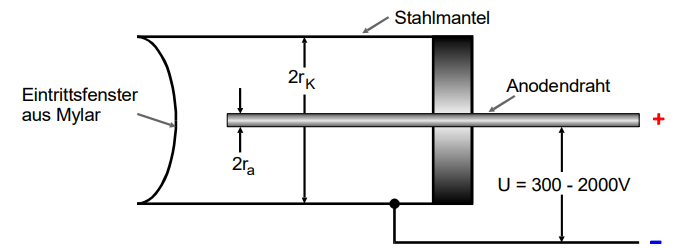
\includegraphics[scale=0.4]{pics/Aufbau.png}
    \caption{Querschnitt eines Endfenster-Zählrohrs [1]}
    \label{fig:aufbau}
  \end{figure}
Es besteht aus einem Kathodenzylinder und einem darin axial verlaufenden Anodendraht. Im inneren befindet sich ein Gasgemisch.
Beim anlegen einer äußeren Spannung entsteht ein radialsymmetrisches Feld. Ein geladenes Teilchen, welches in das Zählrohrvolumen eindringt,
wird sich solange durch den Gasraum bewegen, bis seine Energie durch Ionisationsakte aufgebraucht ist. 
Es werden freie Elektronen und Ionen erzeugt. Die Anzahl der entstehenden Elektronen ist dabei Proportional zur Energie des einfallenden Teilchens.
\begin{figure}
    \centering
    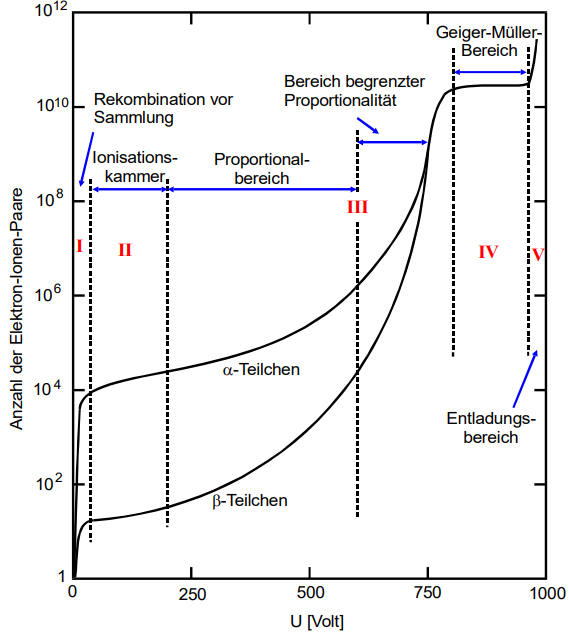
\includegraphics[scale=0.6]{pics/Elektronen.png}
    \caption{Detektierte Elektronen in Abhängigkeit von der Zählrohrspannung [1]}
    \label{fig:Elektronen}
  \end{figure}
In Abbildung \ref{fig:Elektronen} ist erkennbar, dass die Anzahl der erzeugten Elektronen von der Zählrohrspannung $U$ abhängt.
Dabei werden fünf Bereiche unterschieden. Im ersten Bereich ist die angelegte Spannung nicht ausreichend, damit alle Elektronen den Draht erreichen, da viele 
durch Rekombination verloren gehen.
Bei ausreichender Spannung ist der Ionisationsstrom proportional zur Energie der einfallenden Strahlung.
Dieser Bereich wird als Ionisationskammer bezeichnet.
Jedoch kann diese Kammer praktisch nur für hohe Strahlintensitäten genutzt werden, da die Ströme sehr gering sind.
Der dritte Bereich wird bezeichnet als Proportionalitätsbereich bezeichnet. In diesem Bereich haben die 
Elektronen genügend Energie um durch Stoßionisation ihrerseits ionisieren zu können.
Die erzeugten freien Elektronen können ebenfalls ionisieren. Die Anzahl an freien Elektronen steigt damit lawinenartig an. Dieser Prozess wird als
Townsend-Lawine bezeichnet. Die gesammelte Ladung $Q$ ist Proportional zur Primärteilchenenergie. Somit lässt sich das Proportionalitätsrohr zur Energiemessung der
einfallenden Strahlung verwenden.
Bei weiterer Erhöhung der Betriebsspannung wird die Ladung $Q$ unabhängig von der Primärionisation. 
Die Ladung hängt nur noch vom Volumen und der Spannung ab. Dieser Effekt kommt durch die Entstehung von ungeladenen UV-Photonen, die sich auch Senkrecht zum E-Feld
ausbreiten können, wodurch weitere Lawinen im gesamten Zählrohrvolumen ausgelöst werden. 
Das Geiger-Müller-Zählrohr kann nur noch zur Intensitätsmessung benutzt werden.
Der lineare Anteil in diesem bereich wird als Plateau bezeichnet. Dabei weisen hochwertigere Geiger-Müller-Zählrohre ein längeres und flacheres Plateau auf.
Wird die Spannung weiter erhöht, wird durch ein einzelnes Teilchen die Dauerentladung gezündet. Dies zerstört schnell das Zählrohr.